\documentclass[10pt,conference,compsocconf]{IEEEtran}

%\usepackage{times}
%\usepackage{balance}
\usepackage{url}
\usepackage{graphicx}	% For figure environment
\usepackage{booktabs}

\usepackage{subcaption}
\usepackage{hyperref}
\usepackage{pdfpages}

\clubpenalty=-100
%\windowpenalty=-100
\displaywidowpenalty=-100 
\linepenalty=5000
\clubpenalty=10000
\widowpenalty=10000
\displaywidowpenalty=10000

% Problems of Task:
% - small dataset => gmaps & augmentations
% imbalanced dataset => balanced losses?
% Noisy dataset => losses, pre-trained models
% dual task definition

% Baselines:
% 1. UNet encoder on patches
% 2. UNet encoder on pixels

% Structure
% - gmaps dataset
% - unet
% - augmentations
% - ensemble
% - fine-tuning the model on the training dataset
% - ResNet pre-trained on ImageNet
% - early stopping
% - dataset normalization (per city)
% - focal loss

\begin{document}
\title{Road Segmentation: patch-wise vs pixel-wise models}

\author{
  Felix Sarnthein, Rares Constantin, Juraj Micko and Aashish Kumar Singh\\
  Group: GeeseSquad \\
  Department of Computer Science, ETH Zurich, Switzerland
}

\maketitle

\begin{abstract}
  The task of image segmentation has been widely explored, and a range of algorithms find a wide domain of usage nowadays. Satellites produce a massive amount of high-quality images across all landscapes and potentially enable machine map generation. However, human labeled data is usually expensive to produce and labels might be noisy. Road Segmentation is the problem of dividing each image into regions that contain roads and regions that do not. We explore patch-wise and pixel-wise approaches to road segmentation in a small dataset with noisy labels.
\end{abstract}

\section{Introduction}
This work aims to carry out the task of road segmentation via deep neural networks -- exploring potential architectures and analyses of the results. Given a set of 400x400 RGB aerial images, we are asked to classify each 16x16 pixel patch as either containing road or background. A patch is defined as containing road if more than 25\% of its pixels are marked as road in a pixel-wise segmentation mask. Therefore, the task can be seen as a pixel-wise classification or as a patch-wise regression which aims at predicting the ratio of road pixels in a patch. We explore patch-wise and pixel-wise approaches of this dual task definition, identify difficulties of the dataset and ultimately propose a strategy to solve them.

Section 2 of this paper discusses some related works published that aim at the task of road segmentation in aerial images. Section 3 describes the techniques involved in additional training data acquisition and data pre-processing. It further presents details of the model architectures implemented as a part of the solution. Section 4 discusses the results of our experiments. Section 5 discusses the experiments and results and further sheds light on potential future work.
% introducing the task, the provided data, etc


\section{Related Work}
In this section, we are briefly going over some of the previous deep learning techniques for the task of road segmentation in aerial images.

One of the standard deep learning methods for tackling semantic segmentation problems is using a fully convolutional neural network (FCNN). This method involves learning the images' features in a compressed latent space, followed by an upsampling phase to get the predictions in the input space. Some of the papers that adopt the FCNN approach for road segmentation in satellite images are the ones by Henry et. al~\cite{fcnn-road-segmentation-1} and Buslaev et al.~\cite{fcnn-road-segmentation-2}.

An extension of FCNN for semantic segmentation was proposed by Ronneberger et al.~\cite{unet}. This approach revolves around an architecture called U-Net, which consists of "a contracting path to capture context and a symmetric expanding path that enables precise localization". Utilizing transpose convolutions in the decoder and skip connections to get contextual information from low-level layers, the U-Net network outperforms previous architectures by generating sharper segmentation masks. Even though the U-Net was initially designed for biomedical images, researchers such as Hou et al.~\cite{unet-road-segmentation} have managed to adapt the architecture for the task of road segmentation.

One advantage of Convolutional Networks is the weight-sharing which heavily regularizes the model, making it easier to train. However, this comes at the cost of highly local features: On the one hand, neighboring pixels will always have similar features, making it more difficult to produce rigid boundaries like in segmentation. On the other hand, the context covers only parts of the image, making it more difficult to model global structures like roads. The recently proposed Vision Transformer (ViT) \cite{vit} is a novel image model without convolutions. It was extended to work with semantic segmentation for example in the Segmenter acrchitecture \cite{segmenter} and STEGO \cite{stego}.
%% TODO: Transformer, DINO, STEGO

\section{Proposed Method}
We identify four difficulties with the task at hand. Most prominently, the 144 images constitute a very \emph{small dataset} which means that even for a simple neural network, the problem is heavily over-parameterized. Secondly, the dataset is \emph{imbalanced}, with only about 14\% of the pixels belonging to the road class. Furthermore, the data is \emph{noisy} as the definition of roads is not very precise, and human annotation is not always coherent. Finally, although we are confronted with a segmentation task, the final evaluation is on patch-wise averages. This gives rise to a \emph{dual task} definition: either a binary classification of pixels or a logistic regression of patch-wise aggregates. In this section, we evaluate five different components specifically designed to tackle the difficulties of the task: Baselines, Losses, Architectures, Augmentations, and Additional Dataset.
% \begin{itemize}
%     \item Baselines
%     \item Losses
%     \item Architectures
%     \item Augmentations
%     \item Additional Dataset
% \end{itemize}

\subsection{Baselines}
As baselines, we consider two Convolutional Neuronal Networks (CNN) inspired by the original UNet architecture~\cite{unet} trained to minimize a binary cross-entropy (BCE) loss. Both consist of blocks with two padded 3x3 convolutions, ReLU activation functions, and batch normalization. An encoder consists of five such blocks. After every block, the resolution is halved with a 2x2 max-pooling operation while the number of channels doubles. Hence, an initial 3x400x400 input image is encoded layer-by-layer into a 1024x25x25 activation map.\

A decoder is applied to this 25x25 activation map in the U-Net to produce a 400x400 output map. The decoder consists of the same blocks as the encoder but uses learnable transposed convolutions to upsample the resolution. Intermediate activation maps of the encoder are passed directly to the decoder, building so-called skip-connections.\

We evaluate two baselines, one for each interpretation of the task description: a standard encoder-decoder UNet for pixel-wise classification and an encoder-only CNN for patch-wise logistic regression. The encoder-only architecture applies a 1x1 convolution to the intermediate activation map, which yields the 25x25 patch-wise output map.

\subsection{Losses}
Due to the class imbalance of 18\% on patches (14\% in pixels), a classifier always predicting background will already achieve 82\% accuracy. For evaluation of such a task, the weighted F1 score is a more robust metric with respect to label imbalance since it combines the precision and recall of both the negative and positive classes by aggregating them according to their class weight. The standard BCE loss computes a pixel- or patch-wise error and aggregates it over all 625 patches and 8 images in a batch. Since the background class is over-represented in most batches, one would expect the gradient of the BCE loss to be skewed towards the negative class. An optimal solution would then trade-off precision for recall, which would result in a less optimal f1w score.

To counteract this behavior, we implement a balanced BCE (BBCE) loss, which rebalances the weight of the negative and positive samples. In particular, we compute the class imbalance for every patch as if the classes were balanced:$$bbce = \frac{1}{2 N^+ N^-} 
(\sum_{i^+ \in N^+} N^- ce_{i^+}  + \sum_{i^- \in N^-} N^+ ce_{i^-})
$$

Another problem of the dataset is label noise, which adds wrong optimization pressure due to incoherent labels: something might be classified as a road but is not, or vice-versa. The Focal loss \cite{focalloss} addresses this issue for binary classification by down-weighing samples far away from the decision boundary using a discount factor $\gamma$. We extend the focal loss to the logistic regression setting for patch-wise predictions as shown in  \autoref{fig:losses}.

\begin{figure}[ht!]
    \centering
    \begin{subfigure}{0.324\columnwidth}
        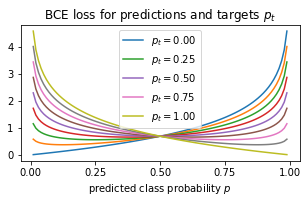
\includegraphics[width=1\textwidth]{pictures/bce.png}
    \end{subfigure}
    \begin{subfigure}{0.324\columnwidth}
        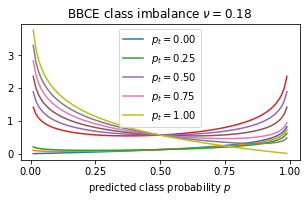
\includegraphics[width=1\textwidth]{pictures/bbce.png}
    \end{subfigure}
    \begin{subfigure}{0.324\columnwidth}
        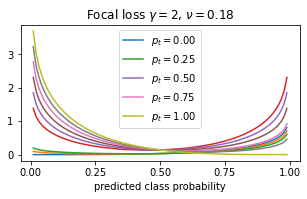
\includegraphics[width=1\textwidth]{pictures/focal.png}
    \end{subfigure}
    \caption{Comparing BCE, BBCE, and Focal loss for patch-wise logistic regression. The BBCE applies less optimization pressure to samples with $p_t < 0.25$. The Focal loss down-weighs predictions far away from $p_t$. Best viewed on screen.}
    \label{fig:losses}
\end{figure}

\subsection{Architectures}
Using pre-trained models is a different approach to handling small datasets with noisy and imbalanced data. The gold standard for pre-trained CNNs are Residual Networks (ResNets) \cite{resnet} pre-trained on ImageNet \cite{imagenet}. Like the U-Net encoder, ResNets consists of five blocks, but each block has a residual connection and possibly more convolutions. The timm library \cite{timm} provides implementations and Imagenet pre-trained ResNets, which we modify for our needs. In particular, we use a ResNet-D Variant \cite{resnet-tricks} which features a deep stem, i.e., a block of 3x3 convolutions instead one 7x7 convolution is applied to the input image, and change the initial stride from 2 to 1. We motivate this by the fact that -- as opposed to object detection -- in segmentation tasks, knowledge about high-resolution features is important. As an additional benefit, the modified ResNet-D encoder now produces 25x25 feature maps, which we directly use for patch-wise predictions. For pixel-wise predictions, we implement a ResNet decoder as an inverted ResNet. Aiming to follow the encoder structure as closely as possible, we insert transposed convolutions between the residual blocks and add skip-connections from layers of the same stride similar to the baseline U-Nets. We compare the sizes of all evaluated architectures in \autoref{tab:arch_sizes}.

In vision transformers, an image is usually embedded into patches of 16x16 pixels and transformed through a multi-layer attention mechanism, making it very suitable for our patch-wise regression task. This theoretically allows for global context and pattern-specific activation maps. Although ViTs are not size-invariant by default, we find that the self-supervised training technique DINO \cite{dino} also works for a size of 400. We evaluate the small version of the ImageNet pre-trained DINOViT for patch-wise logistic regression called dinovits, similar to STEGO \cite{stego}.
%We empirically find, that ViTs are by default not size invariant (due to overfitting to the positional encodings) which makes it more difficult to apply a pre-trained model on images of size 400. However, we find that the self-supervised training technique DINO \cite{dino} uses multiple sizes in training and is size invariant. We evaluate the small version of the Imagenet pre-trained DINOViT for patch-wise logistic regression called dinovits, similar to \cite{stego}.

\begin{table}[ht!]
    \centering
    \begin{tabular}{l|r|r}
        \toprule
        size & patch-wise & pixel-wise \\
        \midrule
            unet        & $18.8 \cdot 10^6$ & $ 31.0 \cdot 10^6$ \\
            resnet18d   & $11.2 \cdot 10^6$ & $ 16,3 \cdot 10^6$\\
            resnet50d   & $23,5 \cdot 10^6$ & - \\
            dinovits    & $21,6 \cdot 10^6$ & - \\
        \bottomrule
    \end{tabular}
    \caption{Size of evaluated architectures in comparison.}
    \label{tab:arch_sizes}
\end{table}



% - Model capacity for sparse data
% - context size
% - residual connections better to optimize => resnets
% - Noise: pre-trained backbone => frozen encoder
% - model output => patchwise / pixelwise?
% - ViTs: better context, difficult to train

\newpage
\subsection{Augmentations}
To avoid overfitting due to the small dataset size and improve the model's robustness, we have adapted a training strategy based on augmentations, similar to the one presented by Ronneberger et al.~\cite{unet}. Thus, we chose to preprocess images by augmenting them dynamically during training using the Albumentations library~\cite{albumentations}. \autoref{fig:example-augmentation} illustrates the transformations an image undergoes during our augmentation process. Each transformation has an independent probability of being applied (e.g., 0.5) and falls into one of the three different categories of transformations we defined: color mutations, affine transformations, and distortions.

% \begin{figure}[ht]
%     \centering
%     \begin{subfigure}{0.495\columnwidth}
%         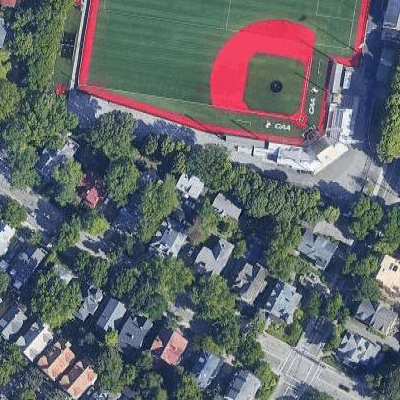
\includegraphics[width=.9\textwidth]{pictures/img_33.png}
%         \label{fig:example-augmentation-original}
%         \caption{original}
%     \end{subfigure}%
%     \begin{subfigure}{0.495\columnwidth}
%         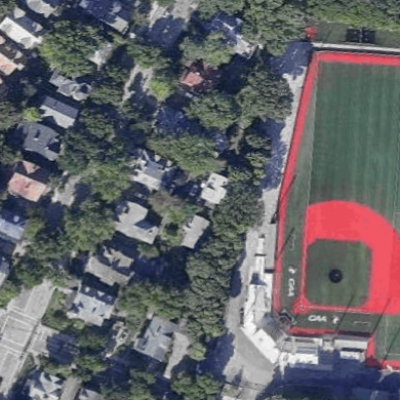
\includegraphics[width=.9\textwidth]{pictures/img_33_augmented.png}
%         \label{fig:example-augmentation-augmented}
%         \caption{augmented}
%     \end{subfigure}
%     \captionsetup{width=0.9\columnwidth}
%     \caption{An example of an image from the training set and a corresponding augmentation.}
%     \label{fig:example-augmentation}
% \end{figure}

\noindent\textbf{Color mutations --} The role of the color mutations is to expand the color distributions of the training images so that they cover the properties of the images used for validation and testing. Hence, we randomly apply different filters and modify certain color attributes of the training images, such as: hue, saturation, brightness, and contrast change, as well as Gaussian noise addition. All of these mutations' ranges were carefully selected so that the images' results still look natural.

\noindent\textbf{Affine transformations --} By applying affine transformations to the input images, the model learns to be invariant to them, increasing overall performance. We use horizontal and vertical flips, transposes, and 90$\pm$10 degrees rotations. Not utilizing all degree values when rotating the images can be justified by the big empty spots that appear in every corner in the case of the excluded degree values. 

\noindent\textbf{Distortions --} To further improve the robustness of the model with respect to small deformations, we apply different types of subtle distortions to the images, such as: grid distortion, optical distortion, and elastic transform. To avoid generating images with unreal features, a maximum of one distortion is used at a time when augmenting an image. We apply a center crop followed by a resizing to the original size to remove potential artifacts at the border.
%Furthermore, to remove the borders that appear emerge during the process, we also perform a center crop, removing 10 pixels from each side. In the end, the image is resized to the original resolution for consistency.

\subsection{Additional Dataset}
While augmentations increase the variability in input images, they do not introduce more variability in the structure of roads. To further improve generalization, we create a much larger dataset by gathering additional satellite images containing roads using the Google Maps API~\cite{google-maps-api}.
%The provided training set contains only 144 images, which are clearly not sufficient for creating a powerful model with high generalization properties. In order to overcome this issue, we created a much larger dataset to train our models on, by gathering additional satellite images containing roads using the Google Maps API~\cite{google-maps-api}.

Utilizing the Maps Static API service, we selected areas from multiple US cities, which, empirically, have a similar appearance to the provided dataset. Precisely, we chose similar areas of the same cities as a team that previously participated in this competition in 2020~\cite{daniCh8-road-segmentation-eth-cil-2020}. The numbers of images for each city were chosen proportionally to their corresponding area, resulting in 12,000 image-label pairs in total, covering a total area of $7,335\, \mathrm{km}^2$. The exact distribution of images in this dataset is as follows: Los Angeles (3,271 images), Chicago (4,067 images), Houston (1,735 images), Phoenix (2,470 images), Philadelphia (235 images), San Francisco (112 images) and Boston (110 images). 
% \begin{figure}
% \centering
% \begin{subfigure}{.5\linewidth}
%   \centering
%   \includegraphics[width=.9\linewidth]{pictures/los_angeles_1849.png}
%   %\caption{A subfigure}
%   \label{fig:gmaps_sample_image}
% \end{subfigure}%
% \begin{subfigure}{.5\linewidth}
%   \centering
%   \includegraphics[width=.9\linewidth]{pictures/los_angeles_1849_mask.png}
%   %\caption{A subfigure}
%   \label{fig:gmaps_sample_mask}
% \end{subfigure}
% \caption{A satellite image (left) and its corresponding label (right) from our Google Maps dataset}
% \label{fig:gmaps_sample}
% \end{figure}
%\autoref{fig:gmaps_sample} displays an example of an image-label pair in our dataset. 
Satellite images were downloaded with a constant zoom level and by specifying i.i.d. generated coordinates of centers within each region. 
%Coordinates were generated using a seeded generator to enable reproducibility. For each satellite image, we downloaded a corresponding black and white mask image to be used as pixel-level labels. 
To generate the image masks, we set up a custom map style in the Google Cloud Console, configuring the visibility of map features (i.e., roads, landscape, pathways, road widths, etc.) on a black background.

\noindent\textbf{Normalization}
Given that the different cities represent different data distributions, we apply per-city data normalization as a pre-processing step. For every city, we once compute the channel-wise statistics of all pixels marked as roads. When loading the images, we subtract the channel-wise mean and divide it by the channel-wise standard deviation. This means that the distributions of road pixels are now close to the standard distribution, while the overall statistics are more irregular. We refer to \autoref{fig:distr} and \autoref{fig:normalized_viz} in the Appendix for more details.


%\noindent\textbf{Fine-tuning --} Since we are utilizing the newly created dataset for training, we need to adapt our models to the target domain. To do so, we fine-tuned our best models on the original training set. To be more exact, we utilized this entire set of images as validation when training on the google maps images and further split it into a training and a validation set for fine-tuning, with a 9:1 ratio.

\section{Experiments and Results}
%To find the best configuration for our model, we conducted an ablation study. To save resources, most of our experiments were performed on the small dataset. For reference, all our models were trained using AdamW~\cite{adamw}, which is an improved variant of the Adam optimizer with weight decay. The default learning rate was set to $1\mathrm{e}{-3}$, and the batch size was set to 8, for both training and evaluation. After all the experiments were finalized, we selected the best options from each set of experiments in order to build multiple models which produce satisfactory results. Moreover, to obtain the final predictions for the competition, we create an ensemble from the predictions of our best performing models, using a weighted voting scheme
We compare all four different strategies to our two Baselines. In all cases, we train on a training split of 129 images using AdamW \cite{adamw} with default parameters and a batch size of 8. We evaluate on a validation split of 15 carefully selected images, measuring the weighted F1 accuracy (F1W) score. We train for 100 epochs and apply early-stopping on the highest validation F1W score for patch-wise predictions. In the special case of augmentations, we train for 250 epochs. When training on the Google Maps data, we validate on all 144 original training images.
% -- Ablation study: what experiments we have done and their results
% -- Show both quantitative and qualitative results (metrics and predictions)

\subsection{Losses}
We observe that the balanced losses are much more unstable to train than the standard BCE. While initially maintaining higher recall and lower precision, they converge towards the baseline values but with lower overall performance. This is also reflected in the evaluation in \autoref{tab:results_table_losses}.
\begin{table}[ht!]
    \centering
    \begin{tabular}{l|rr|rr}
        \toprule
        \multicolumn{1}{c}{} &
        \multicolumn{2}{c}{patch-wise} &
        \multicolumn{2}{c}{pixel-wise} \\
        \multicolumn{1}{c}{\textbf{experiment}} &
        \multicolumn{1}{c}{\textbf{F1W}} &
        \multicolumn{1}{c}{\textbf{epoch}} &
        \multicolumn{1}{c}{\textbf{F1W}} &
        \multicolumn{1}{c}{\textbf{epoch}} \\
        \midrule
            BCE & \textbf{0.88} & 97 & \textbf{0.883} & 94 \\
            BBCE & 0.869 & 67 & 0.865 & 99 \\
            Focal & 0.669 & 47 & 0.84 & 98 \\
        \bottomrule
    \end{tabular}
    \caption{Different losses compared to the two baselines.}
    \label{tab:results_table_losses}
    \vspace{-0.5cm}
\end{table}

\subsection{Architectures}
In \autoref{tab:results_table_architectures}, we observe that the ResNet18-D architectures perform similar to the baselines when trained from scratch, although they have fewer parameters. Furthermore, we observe the ImageNet pre-trained models increase the performance by 1-2\%. We evaluate the feature quality of pre-trained models by training the decoder only and observe that those features achieve competitive performance, especially for pixel-wise predictions where the decoder is more complex. Unfortunately we were only able to evaluate the superior performance of ViT features. Training ViTs seems to require a complex optimization procedure that we could not reproduce.

\begin{table}[ht!]
    \centering
    \begin{tabular}{l|rr|rr}
        \toprule
        \multicolumn{1}{c}{} &
        \multicolumn{2}{c}{patch-wise} &
        \multicolumn{2}{c}{pixel-wise} \\
        \multicolumn{1}{c}{\textbf{experiment}} &
        \multicolumn{1}{c}{\textbf{F1W}} &
        \multicolumn{1}{c}{\textbf{epoch}} &
        \multicolumn{1}{c}{\textbf{F1W}} &
        \multicolumn{1}{c}{\textbf{epoch}} \\
        \midrule
            U-Net        & 0.88 & 97 & 0.883 & 94 \\
            ResNet18d   & 0.882 & 29 & 0.884 & 93 \\
            ResNet18d*  & 0.727 & 99 & 0.878 & 67 \\
            ResNet18d** & 0.892 & 53 & \textbf{0.893} & 18 \\
            ResNet50d   & 0.879 & 98 & - & - \\
            ResNet50d*  & 0.741 & 100 & - & - \\
            ResNet50d** & \textbf{0.894} & 87 & - & - \\
            DinoViTs*   & 0.790 & 100 & - & - \\
        \bottomrule
    \end{tabular}
    \caption{Different architectures compared to the two baselines. 
    *Imagenet pre-trained backbone: training decoder only  
    **Imagenet pre-trained backbone: fine-tuning end-to-end}
    \label{tab:results_table_architectures}
\end{table}

\subsection{Augmentations}
In \autoref{tab:results_table_augmentations} we observe that augmentations increase the generalization abilities by 1-2\% and that the group of affine augmentations contributes the most.

\begin{table}[ht!]
    \centering
    \begin{tabular}{l|rr|rr}
        \toprule
        \multicolumn{1}{c}{} &
        \multicolumn{2}{c}{patch-wise} &
        \multicolumn{2}{c}{pixel-wise} \\
        \multicolumn{1}{c}{\textbf{augmentations}} &
        \multicolumn{1}{c}{\textbf{F1W}} &
        \multicolumn{1}{c}{\textbf{epoch}} &
        \multicolumn{1}{c}{\textbf{F1W}} &
        \multicolumn{1}{c}{\textbf{epoch}} \\
        \midrule
            without & 0.886 & 225 & 0.884 & 124 \\
            color\&noise & 0.882 & 412 & 0.871 & 136 \\
            affine & \textbf{0.903} & 271 & \textbf{0.901} & 357 \\
            distortions & 0.897 & 228 & 0.887 & 126 \\
            all & 0.902 & 481 & \textbf{0.901} & 355 \\
        \bottomrule
    \end{tabular}
    \caption{Different augmentations compared to the baseline.}
    \label{tab:results_table_augmentations}
\end{table}

\subsection{Additional Dataset}
In \autoref{tab:results_table_additional_dataset} observe that training on the large Google Maps dataset increases performance by 2\%, of which 1\% is due to the sophisticated normalization strategy.

\begin{table}[ht!]
    \centering
    \begin{tabular}{l|rr|rr}
        \toprule
        \multicolumn{1}{c}{} &
        \multicolumn{2}{c}{patch-wise} &
        \multicolumn{2}{c}{pixel-wise} \\
        \multicolumn{1}{c}{\textbf{training set}} &
        \multicolumn{1}{c}{\textbf{F1W}} &
        \multicolumn{1}{c}{\textbf{epoch}} &
        \multicolumn{1}{c}{\textbf{F1W}} &
        \multicolumn{1}{c}{\textbf{epoch}} \\
        \midrule
            original & 0.88 & 97 & 0.883 & 94 \\
            gmaps & 0.889 & 11 & \textbf{0.894} & 8 \\
            gmaps* & \textbf{0.899} & 7 & \textbf{0.894} & 8 \\
            %gmaps* + fine-tuning & value & epoch & 0.907 & 21 \\
        \bottomrule
    \end{tabular}
    \caption{Models' performance when using the additional dataset for training compared to the one that uses the original dataset.
    *Every dataset is normalized for road pixels to match the standard normal distribution.}
    \label{tab:results_table_additional_dataset}
\end{table}

\subsection{Combining Strategies}
After evaluating the different strategies, select a few combinations to, as shown in \autoref{tab:results_table_final}. The model used for the final Kaggle submission is a voting ensemble of all these models. Using this method, we achieved a final score of \textbf{0.93524} on the platform.
\begin{table}[ht!]
    \centering
    \begin{tabular}{l|rr|rr}
        \toprule
        \multicolumn{1}{c}{} &
        \multicolumn{2}{c}{patch-wise} &
        \multicolumn{2}{c}{pixel-wise} \\
        \multicolumn{1}{c}{\textbf{model}} &
        \multicolumn{1}{c}{\textbf{F1W}} &
        \multicolumn{1}{c}{\textbf{epoch}} &
        \multicolumn{1}{c}{\textbf{F1W}} &
        \multicolumn{1}{c}{\textbf{epoch}} \\
        \midrule
            baseline & 0.88 & 97 & 0.883 & 94 \\
            U-Net & 0.921 & 87+3 & 0.917 & 60 + 27 \\
            ResNet18d & \textbf{0.927} & 79 + 5 & 0.918 & 60 + 4 \\
            ResNet50d & - & - & \textbf{0.922} & 80 + 12 \\
        \bottomrule
    \end{tabular}
    \caption{The scores of models combining the best strategies. All models were trained on the Google Maps images and fine-tuned on the original dataset.}
    \label{tab:results_table_final}
    \vspace{-0.1cm}
\end{table}

\section{Discussion and Future Work}
In our quest to solve the task of training a segmentation model on a \emph{small} and \emph{imbalanced} dataset with \emph{noisy} labels for \emph{patch-wise predictions}, we find that most of our components help to conquer these problems. Most importantly, to solve the dual task, we observe that patch-wise models are competitive with pixel-wise models, but the former perform slightly better in an optimal setting. While specialized losses did not achieve to overcome imbalanced and noisy labels, pre-trained models proved to do so. Using augmentations, an additional dataset with pre-processing and fine-tuning reduced the burden of a small dataset. Finally, creating a voting ensemble of best-performing strategies resulted in a satisfactory Kaggle score.

Our results show the superior feature quality of vision transformers, which suggests looking into these models for patch-wise predictions. For future work, we consider using self-supervised learning to avoid noisy labels. Furthermore, an even larger dataset could be created to get more variability in the structure of roads. Finally, we consider developing a more sophisticated method to produce patch-wise activations from pixel-embeddings instead of simple averaging. For example, an attention mechanism could bridge the gap between the pixel- and patch-wise prediction tasks. 

% -- Discussion of the results and what can be added / changed so we can achieve even better performance?
\begin{figure}[h]
\centering
\begin{subfigure}[t]{.25\linewidth}
  \centering
  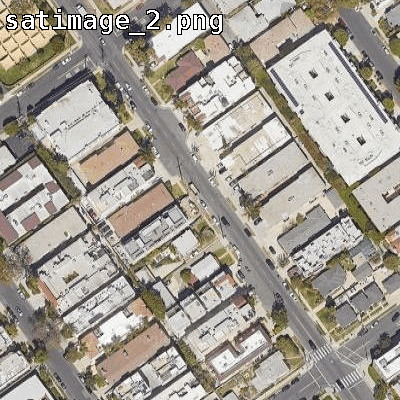
\includegraphics[width=.9\linewidth]{pictures/eval_image.png}
  \caption{\footnotesize Source image}
  \label{fig:patch_diff_image}
\end{subfigure}%
\begin{subfigure}[t]{.25\linewidth}
  \centering
  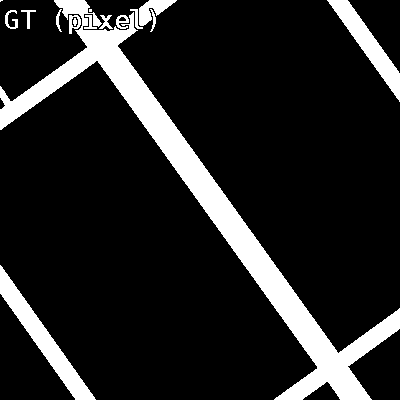
\includegraphics[width=.9\linewidth]{pictures/eval_label.png}
  \caption{\footnotesize Label}
  \label{fig:patch_diff_label}
\end{subfigure}%
\begin{subfigure}[t]{.25\linewidth}
  \centering
  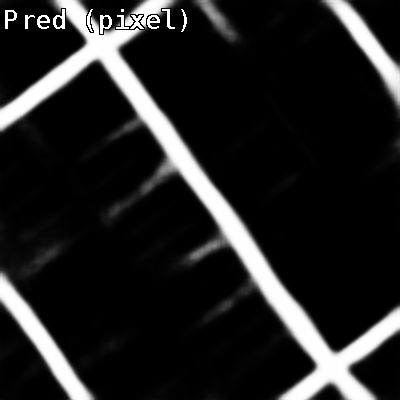
\includegraphics[width=.9\linewidth]{pictures/eval_pred.png}
  \caption{\footnotesize Prediction}
  \label{fig:patch_diff_pred}
\end{subfigure}%
\begin{subfigure}[t]{.25\linewidth}
  \centering
  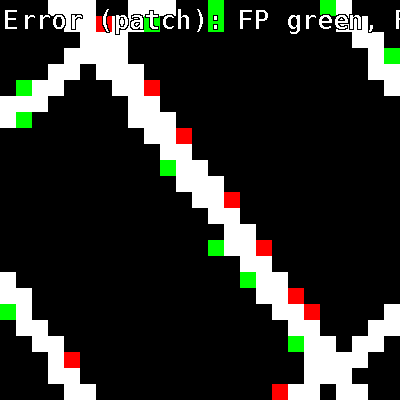
\includegraphics[width=.9\linewidth]{pictures/eval_patch_diff.png}
  \caption{\footnotesize Error type}
  \label{fig:patch_diff_patches}
\end{subfigure}
\caption{Qualitative evaluation of a U-Net model, demonstrating the potential for improvement by ViTs: false positives (green), false negatives (red).}
\label{fig:patch_diff}
\vspace{-0.1cm}
\end{figure}

\section{Conclusion}
Producing accurate segmentation masks for roads in satellite images proved challenging, especially with access to few training examples. Using a multitude of techniques, such as generating a larger dataset for training, creating augmentations, and using transfer learning, we surpassed the performance of the selected baseline models, thus achieving satisfactory results.
% -- Just a wrap up


\newpage
\bibliographystyle{IEEEtran}
\bibliography{road-segmentation}

\newpage

\begin{figure*}[ht]
\section{Appendix}
    \centering
    \begin{subfigure}{0.495\textwidth}
        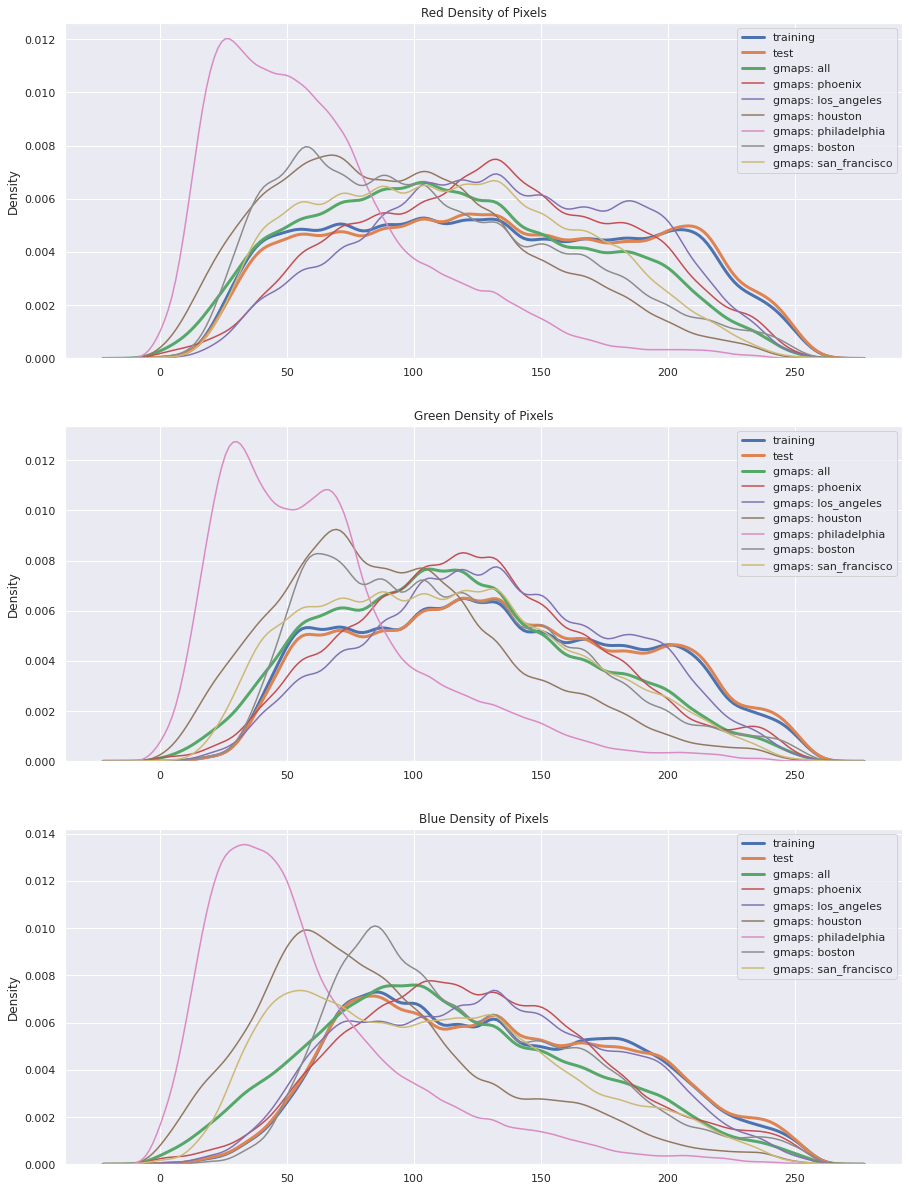
\includegraphics[width=.9\textwidth]{pictures/distr_pixels.png}
        \label{fig:distr_pixels}
        \caption{densities all pixels}
    \end{subfigure}%
    \begin{subfigure}{0.495\textwidth}
        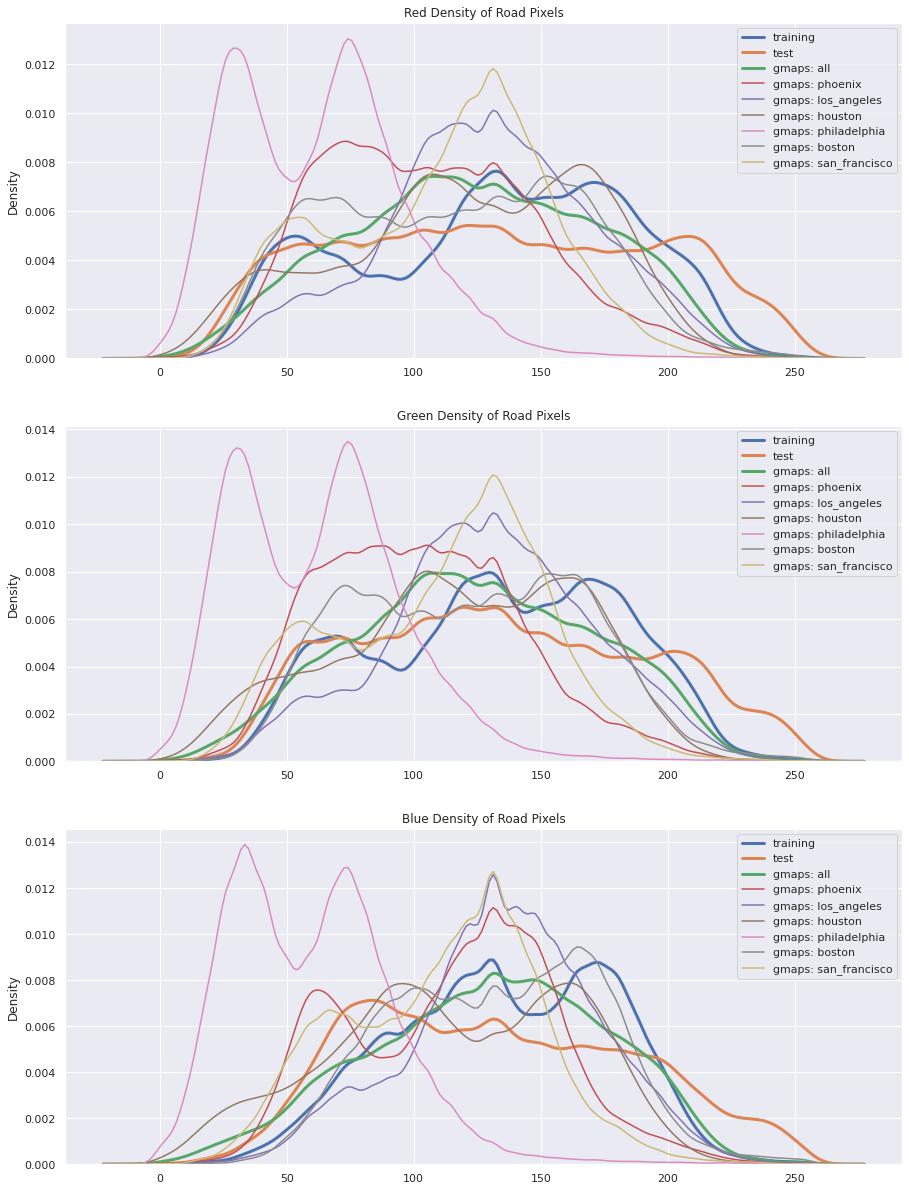
\includegraphics[width=.9\textwidth]{pictures/distr_pixels_road.png}
        \label{fig:distr_pixels_road}
        \caption{densities road pixels}
    \end{subfigure}
    \begin{subfigure}{0.495\textwidth}
        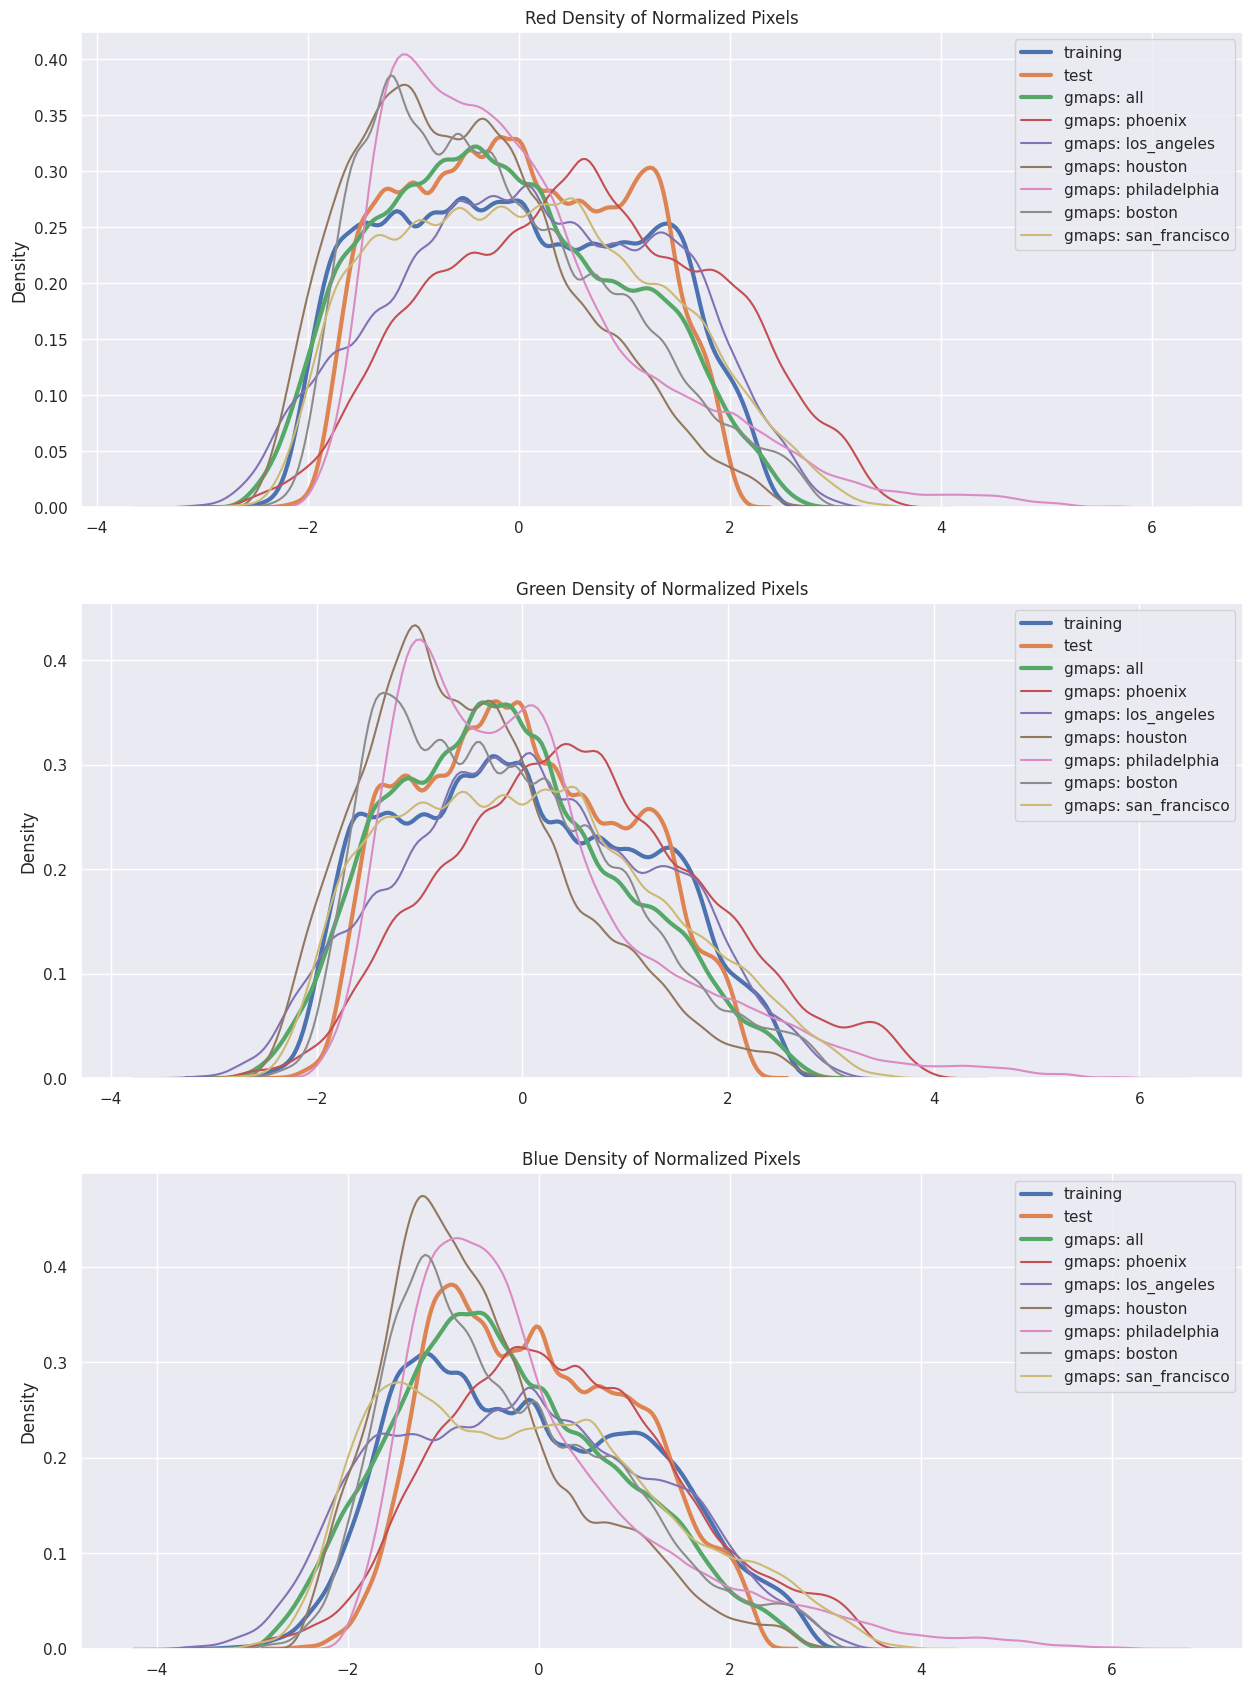
\includegraphics[width=.9\textwidth]{pictures/distr_pixels_norm.png}
        \label{fig:distr_pixels_norm}
        \caption{normalized densities all pixels}
    \end{subfigure}
    \begin{subfigure}{0.495\textwidth}
        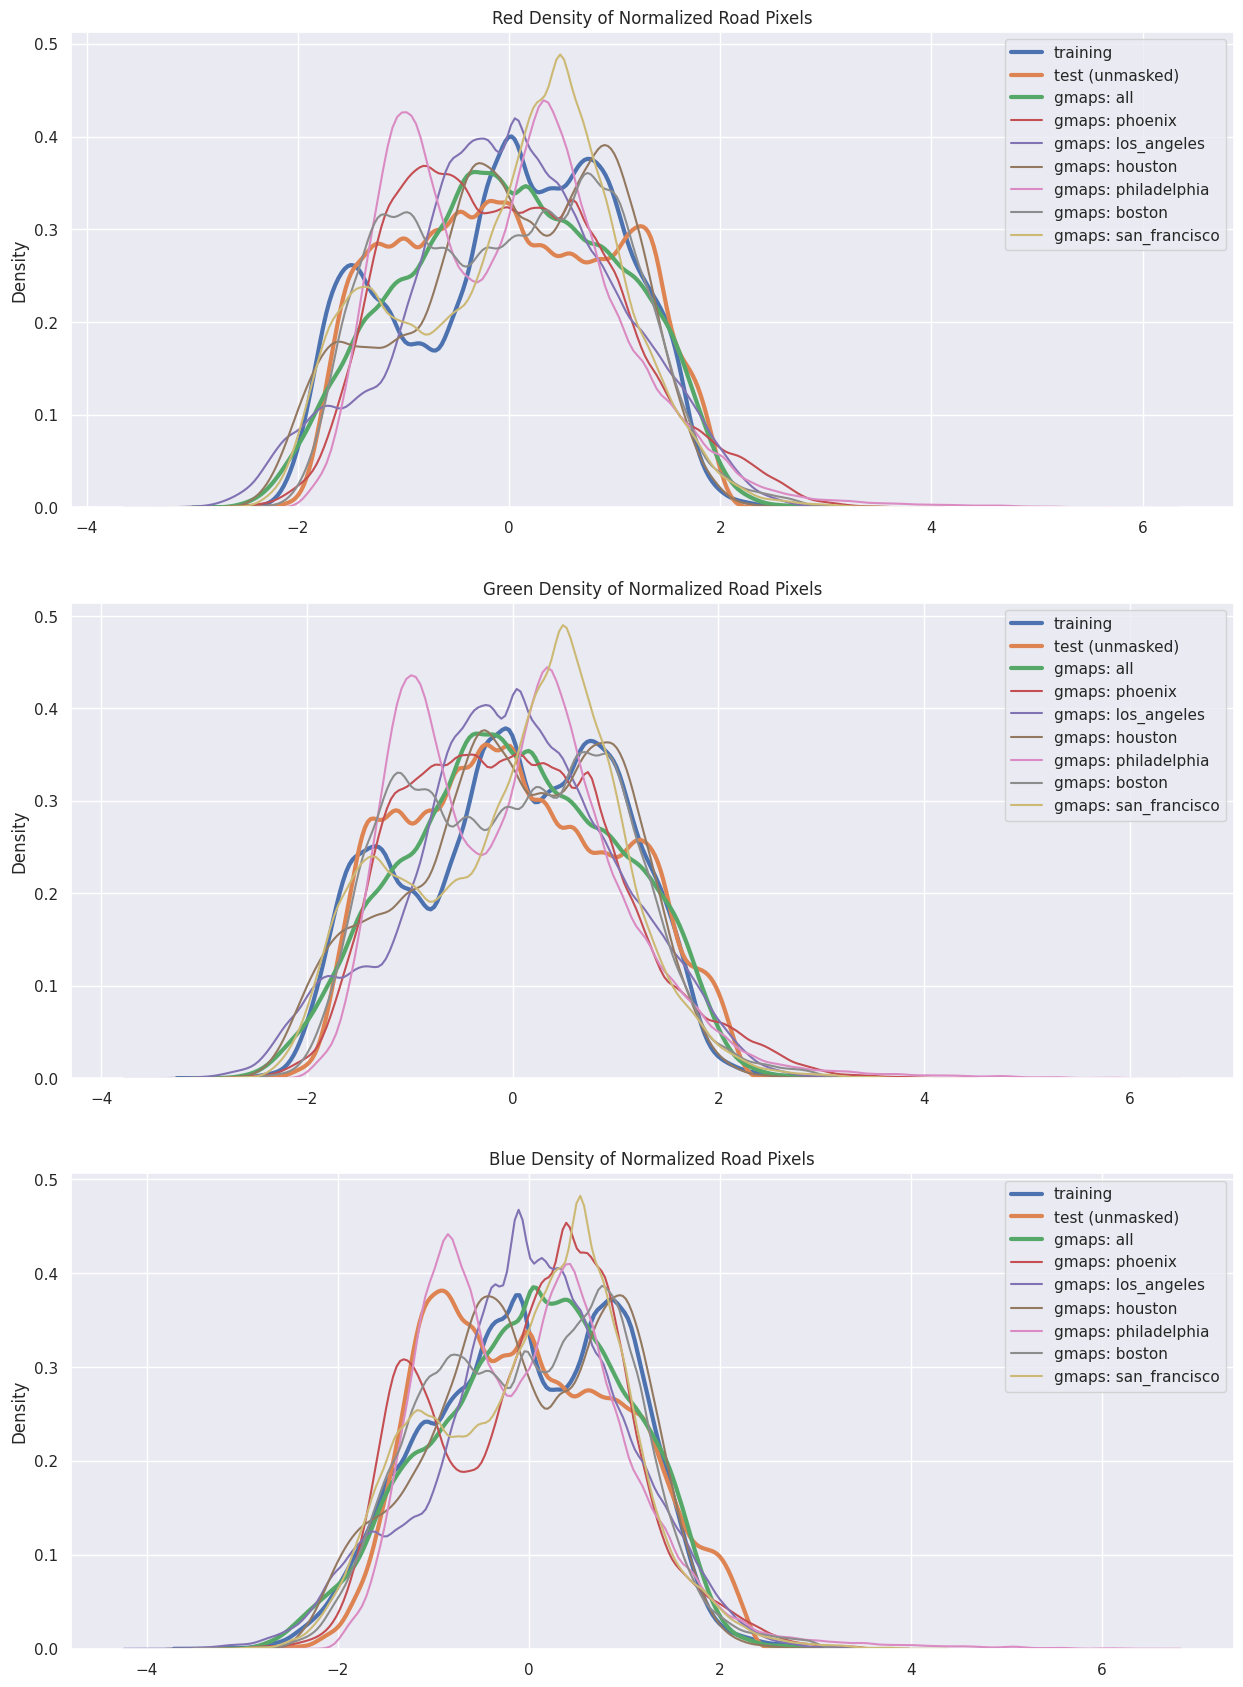
\includegraphics[width=.9\textwidth]{pictures/distr_pixels_road_norm.png}
        \label{fig:distr_pixels_road_norm}
        \caption{normalized densities road pixels}
    \end{subfigure}
    \captionsetup{width=0.9\textwidth}
    \caption{Channel-wise densities of road vs all pixels before and after normalization. Note that normalization according to road statistics causes non-road pixels to be irregularly distributed and potentially easier to separate.}
    \label{fig:distr}
\end{figure*}

\begin{figure*}[ht]
    \centering
    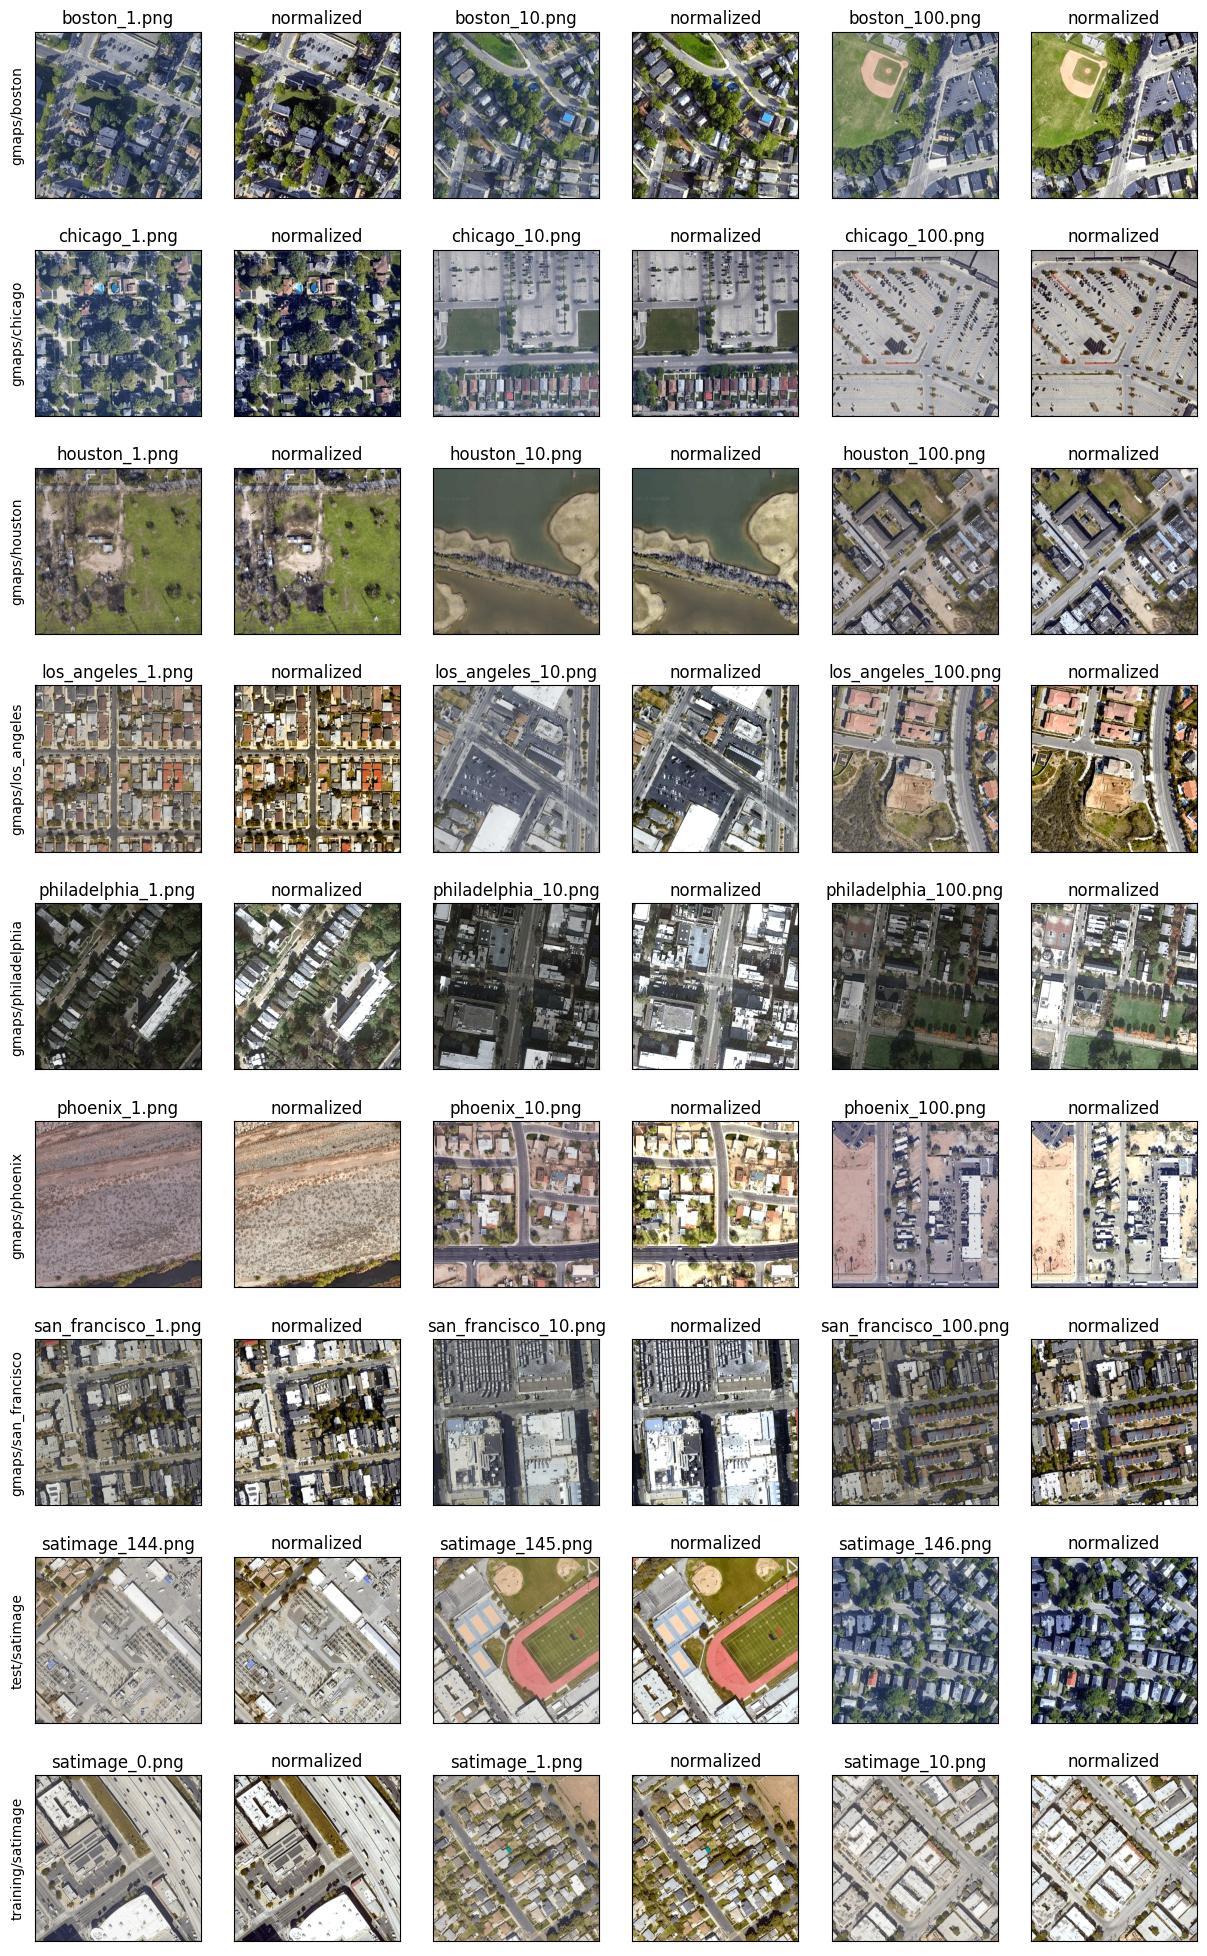
\includegraphics[height=0.9\textheight]{pictures/normalized_viz.png}
    \captionsetup{width=0.9\textwidth}
    \caption{Examples from all cities before and after normalization. Note that road pixels have more similar colors across cities.}
    \label{fig:normalized_viz}
\end{figure*}

\clearpage

\includepdf{Declaration-Originality}
\end{document}
